\documentclass[10pt]{article}
\usepackage[a4paper,margin=1.9cm]{geometry}
\usepackage[utf8]{inputenc}
\usepackage[spanish]{babel}
\usepackage{graphicx}
\usepackage{booktabs}
\usepackage{xcolor}
\usepackage{tikz}
\usetikzlibrary{arrows.meta, positioning, fit}
\usepackage{caption}
\usepackage{float}
\usepackage{amsmath}
\usepackage{enumitem}
\usepackage[colorlinks=true, linkcolor=blue!50!black, urlcolor=blue!50!black, citecolor=blue!50!black]{hyperref}
\usepackage{titlesec}

\setlength{\parskip}{2pt}
\setlength{\parindent}{0pt}
\titlespacing*{\section}{0pt}{8pt}{4pt}
\titlespacing*{\subsection}{0pt}{6pt}{3pt}
\captionsetup{font=small, labelfont=bf}

\definecolor{accent}{HTML}{0284C7}
\definecolor{primary}{HTML}{0F172A}

\title{\vspace{-1.5em}\textbf{\LARGE Sistema Inteligente Adaptativo con Datos No Estacionarios:\\[2pt] \large Detección de Fraude Financiero en E-Commerce}}
\author{
  \normalsize Planificación y Toma de Decisiones en IA (CS5363) --- UTEC 2026-2 \\
  \normalsize Dra. Aurea Soriano-Vargas \& Mg. Robert Buleje \\[4pt]
  \normalsize \textbf{Grupo 7} \\[2pt]
  \normalsize Gálvez Pacori, José Guillermo \quad\textbar\quad Meneses Roncal, Matías Alonso \quad\textbar\quad Ore García, Alejandro Joel
}
\date{\normalsize Proyecto 1}

\begin{document}
\maketitle
\vspace{-2.2em}

\section{Introducción y problema}
El fraude transaccional en e-commerce genera pérdidas superiores a \$48 mil millones anuales a nivel global y más de \$10 mil millones en EE.UU. (FTC, Merchant Savvy), combinando pérdidas directas de capital y fricción operativa por bloqueos erróneos de compras legítimas. Los patrones de fraude cambian continuamente con el tiempo, por lo que un modelo estático pierde efectividad progresivamente. Se propone un sistema inteligente adaptativo de detección de fraude sobre el dataset \textbf{IEEE-CIS Fraud Detection} (Kaggle): 590{,}540 transacciones, 434 columnas, $\sim$26 semanas, 3.499\% de fraude. Se eligió por su drift mixto (evolución gradual de hábitos de consumo + cambios bruscos por nuevas campañas de fraude) y su complejidad (alta dimensionalidad, fuerte desbalance de clases).

\section{Objetivos}
\textbf{General:} implementar un sistema inteligente de detección de fraude transaccional para e-commerce, capaz de evaluar su desempeño en el tiempo y adaptarse al cambio en el comportamiento de los datos.
\textbf{Específicos:} (1) analizar la dimensión temporal del dataset; (2) comparar modelos clásicos y avanzados bajo evaluación cronológica; (3) diseñar la arquitectura del sistema a nivel de componentes; (4) analizar el comportamiento del sistema bajo distintos escenarios de políticas de olvido.

\section{Restricciones}
\textbf{Latencia:} inferencia $<$200\,ms por transacción. \textbf{Información mínima:} el sistema opera solo con los atributos que proveen las pasarelas estándar, sin garantía de datos de identidad completos. \textbf{Consistencia temporal estricta:} ninguna decisión ni reentrenamiento puede usar información de periodos posteriores al evento evaluado.

\section{Diseño del sistema}
\label{sec:diseno}
El sistema se estructura como un pipeline de 5 componentes con un ciclo de retroalimentación (Fig.~\ref{fig:arquitectura}): (1) \emph{Adquisición e integración de datos} (variables transaccionales, de dispositivo/email y de comportamiento); (2) \emph{módulo predictivo} (los 4 modelos candidatos, \S\ref{sec:modelado}); (3) \emph{manejo de incertidumbre} (las predicciones de baja confianza se marcan para revisión, no se resuelven automáticamente); (4) \emph{módulo de decisión} (umbral costo-óptimo, \S\ref{sec:metricas}); (5) \emph{componente de acción} (aprobar o derivar a un analista humano, respetando la restricción de información mínima). Un monitor de drift (ventanas deslizantes sobre F1) dispara el reentrenamiento, y las etiquetas reales retroalimentan la adquisición de datos.

\begin{figure}[H]
\centering
\begin{tikzpicture}[
  node distance=6mm and 6mm,
  box/.style={draw, rounded corners, minimum height=1.05cm, align=center, font=\scriptsize, fill=accent!12, draw=accent},
  boxend/.style={draw, rounded corners, minimum height=1.15cm, align=center, font=\scriptsize, fill=primary, text=white, draw=primary},
  boxsrc/.style={draw, rounded corners, minimum height=1.05cm, align=center, font=\scriptsize, fill=gray!10},
  monitor/.style={draw, dashed, rounded corners, minimum height=0.9cm, align=center, font=\scriptsize, fill=white},
  arr/.style={-{Latex[length=2mm]}, thick, accent}
]
\node[boxsrc, minimum width=1.7cm] (src) {Fuentes de\\datos};
\node[box, minimum width=2.1cm, right=of src] (adq) {\textcircled{\raisebox{-0.9pt}{1}} Adquisición\\e integración};
\node[box, minimum width=2.1cm, right=of adq] (pred) {\textcircled{\raisebox{-0.9pt}{2}} Módulo\\predictivo};
\node[box, minimum width=2.1cm, right=of pred] (unc) {\textcircled{\raisebox{-0.9pt}{3}} Manejo de\\incertidumbre};
\node[box, minimum width=2.1cm, right=of unc] (dec) {\textcircled{\raisebox{-0.9pt}{4}} Módulo de\\decisión};
\node[boxend, minimum width=1.9cm, right=of dec] (act) {\textcircled{\raisebox{-0.9pt}{5}} Acción\\Aprobar / Revisar};

\draw[arr] (src) -- (adq);
\draw[arr] (adq) -- (pred);
\draw[arr] (pred) -- (unc);
\draw[arr] (unc) -- (dec);
\draw[arr] (dec) -- (act);

\node[monitor, below=8mm of pred, xshift=8mm, minimum width=3.6cm] (mon) {Monitor de drift\\(ventanas deslizantes)};
\draw[-{Latex[length=2mm]}, thick, primary, dashed] (mon.north) -- ++(0,2mm) -| (dec.south);
\draw[thick, gray, -{Latex[length=2mm]}] (act.south) |- ++(0,-22mm) -| (src.south);
\node[below=24mm of act, xshift=-9.4cm, font=\tiny, text width=3.2cm, align=center] {feedback: etiquetas reales para reentrenar};
\end{tikzpicture}
\caption{Arquitectura del sistema: 5 componentes, monitor de drift y ciclo de retroalimentación.}
\label{fig:arquitectura}
\end{figure}

\section{Métricas de éxito}
\label{sec:metricas}
\textbf{Técnica:} F1-Score y ROC-AUC evaluados por bloque temporal (F1 $= 2\cdot\frac{P\cdot R}{P+R}$); latencia $<$200\,ms. \textbf{Decisión (negocio):} costo $= \text{FN}\times\$120 + \text{FP}\times\$15$ (monto promedio de fraude y costo de fricción respectivamente). \textbf{Social:} equidad en la tasa de falsos positivos por rango de monto, evitando bloqueos desproporcionados a compras legítimas de bajo ticket.

\section{Modelos}
\label{sec:modelado}
Se comparan 4 modelos: \textbf{Regresión Logística} y \textbf{Random Forest} (línea base clásica) vs. \textbf{LightGBM} y \textbf{XGBoost} (avanzados, boosting).

\section{Análisis y preparación de datos}
El EDA temporal (Fig.~\ref{fig:eda}) muestra que la tasa de fraude \textbf{no es estacionaria}: oscila entre 2.07\% y 5.07\% semanal, con tendencia al alza hacia el final del periodo. Hay un fuerte patrón horario (pico de 10.6\% de fraude entre las 5-9am) y un cambio real en la distribución de \texttt{ProductCD} entre la primera y segunda mitad del periodo (``W'': 70\%$\to$80\%). La cobertura de datos de \texttt{identity} cae abruptamente después de la semana 3 (54\%$\to$15-26\%), reforzando la restricción de información mínima.

\begin{figure}[H]
\centering
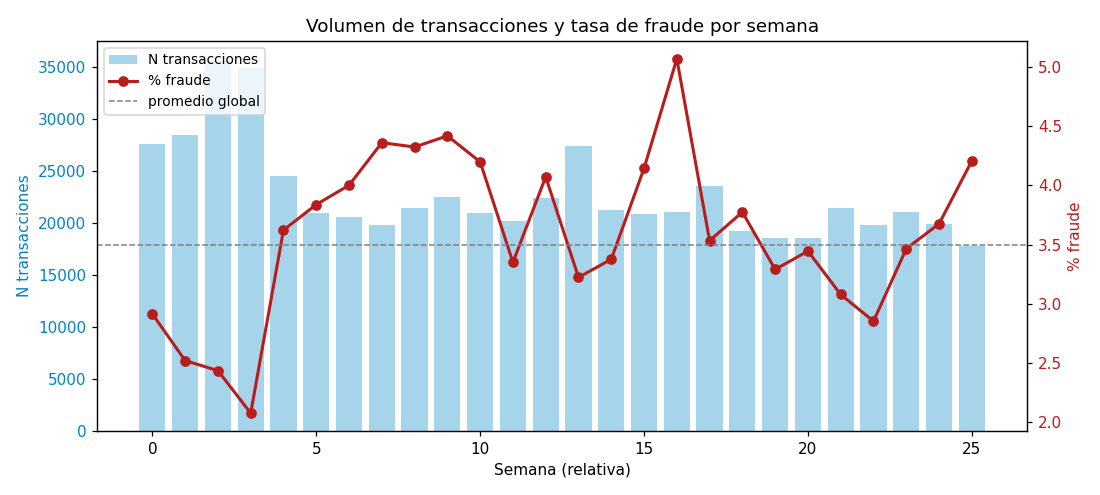
\includegraphics[width=0.92\linewidth]{../figures/01_weekly_volume_fraud_rate.png}
\caption{Volumen y tasa de fraude por semana: no estacionariedad confirmada con datos reales.}
\label{fig:eda}
\end{figure}

\textbf{Preprocesamiento:} las 40 columnas individuales de \texttt{identity} se descartan en favor de un flag \texttt{has\_identity}; nulos numéricos se imputan con $-999$ (constante, sin fuga); categóricas se codifican a enteros; \texttt{TransactionAmt} se winsoriza al percentil 99.5. Se agregan variables de ventana de 24h por tarjeta (\texttt{card1}). El split train/val/test (60/20/20) respeta estrictamente el orden cronológico.

\section{Modelado y evaluación}
La Tabla~\ref{tab:modelos} resume el desempeño en validación con umbral 0.5. XGBoost gana en F1/ROC-AUC, pero con ese umbral su costo de negocio es \emph{peor} que el de LightGBM (alta precisión, bajo recall: cada fraude no detectado cuesta 8$\times$ más que una fricción). Por eso se optimiza el umbral por separado sobre el modelo ganador (Fig.~\ref{fig:umbral}): el óptimo es \textbf{0.07}, no 0.5, con un ahorro del \textbf{28.3\%} en costo de negocio sobre validación.

\begin{table}[H]
\centering\small
\begin{tabular}{lrrrr}
\toprule
Modelo & F1 & ROC-AUC & Costo (umbral 0.5) \\
\midrule
Regresión Logística & 0.239 & 0.851 & \$452{,}265 \\
Random Forest        & 0.370 & 0.888 & \$317{,}595 \\
LightGBM              & 0.415 & 0.917 & \$275{,}100 \\
\textbf{XGBoost}      & \textbf{0.515} & \textbf{0.921} & \$354{,}510 \\
\bottomrule
\end{tabular}
\caption{Comparación de los 4 modelos en validación (umbral por defecto 0.5).}
\label{tab:modelos}
\end{table}

\begin{figure}[H]
\centering
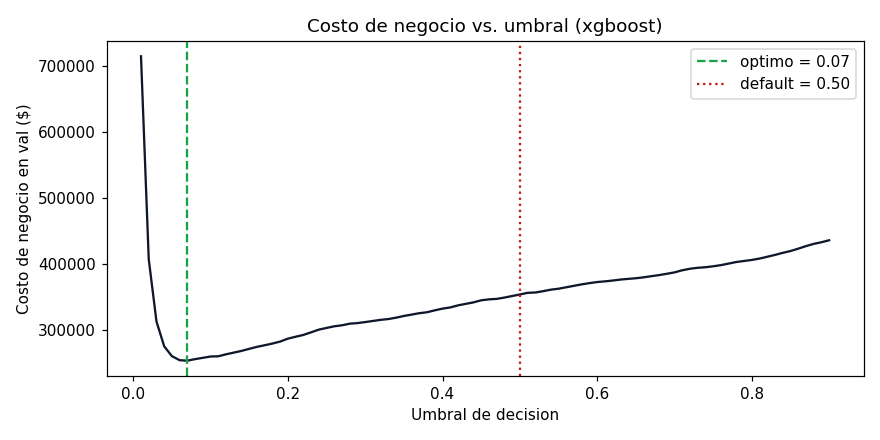
\includegraphics[width=0.92\linewidth]{../figures/06_cost_vs_threshold.png}
\caption{Costo de negocio vs. umbral de decisión (XGBoost): el óptimo es 0.07.}
\label{fig:umbral}
\end{figure}

La importancia de variables está dominada por columnas anonimizadas originales (\texttt{V*}, \texttt{C*}); nuestras variables de ingeniería quedan en posiciones bajas (rango \#187-\#377 de 397) --- un hallazgo honesto: el poder predictivo principal viene de los datos ya provistos, no de las features nuevas.

\section{Evaluación temporal}
Evaluando una sola vez sobre \texttt{test} (nunca antes usado), el desempeño cae respecto a validación: F1 de 0.495 a 0.406 (\textbf{-18\%}), ROC-AUC de 0.921 a 0.886, costo de \$254{,}190 a \$278{,}910. Esta caída \textbf{supera el umbral de alerta del 5\%} definido para disparar el reentrenamiento (\S\ref{sec:drift}). Sin embargo, al dividir \texttt{test} en 8 bloques temporales (Fig.~\ref{fig:degradacion}) no se observa una degradación monótona: el rendimiento oscila y se recupera hacia el final --- la caída real ocurre \emph{entre} periodos (val$\to$test), no como un colapso progresivo dentro de la ventana de test.

\begin{figure}[H]
\centering
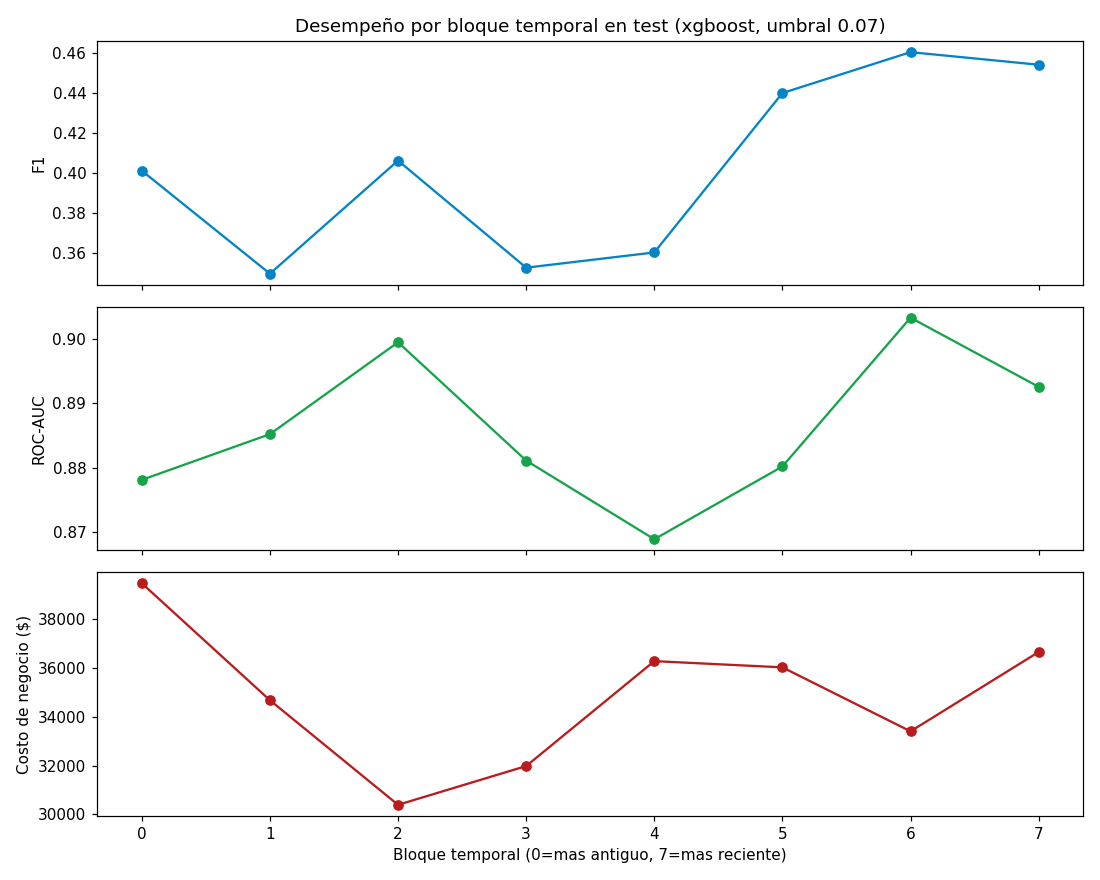
\includegraphics[width=0.92\linewidth]{../figures/07_temporal_degradation.png}
\caption{F1, ROC-AUC y costo por bloque temporal en test: oscilación sin colapso monótono.}
\label{fig:degradacion}
\end{figure}

\section{Detección y adaptación al concept drift}
\label{sec:drift}
Se simulan 5 estrategias de reentrenamiento en 2 cortes temporales (día 120 y 150 sobre la línea de tiempo completa), evaluando cada una sobre el mismo bloque futuro de 20 días: sin olvido (todo el historial), ventanas deslizantes de 30/60/90 días (Escenario A), y time-decay con vida media de 30 días (Escenario B). La Fig.~\ref{fig:drift} resume los resultados: \textbf{``sin olvido'' nunca es la mejor estrategia} en ninguno de los dos cortes (en el corte 150 es la peor, \$123{,}090 vs. \$117{,}735 de la ventana de 30 días), pero \textbf{ninguna ventana gana en ambos cortes} --- el tamaño óptimo de ventana también parece cambiar con el tiempo.

\begin{figure}[H]
\centering
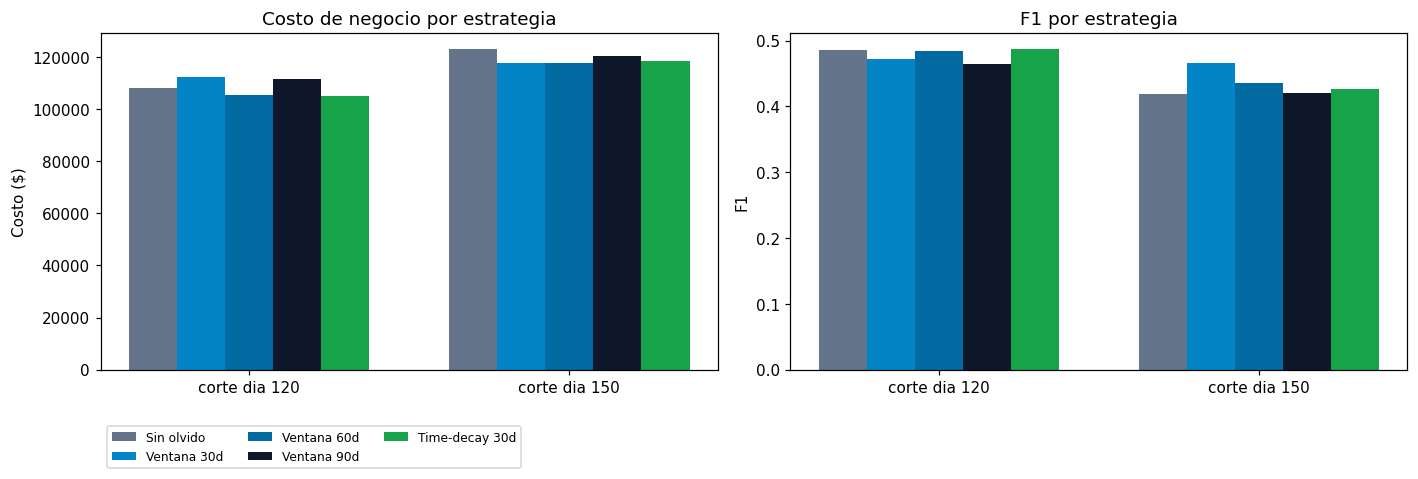
\includegraphics[width=0.98\linewidth]{../figures/08_drift_scenarios_comparison.png}
\caption{Costo y F1 por estrategia de olvido, en dos cortes temporales distintos.}
\label{fig:drift}
\end{figure}

\subsection*{Reflexión crítica}
Un sistema que fija un único tamaño de ventana ``para siempre'' puede quedar mal calibrado si la naturaleza del drift cambia; automatizar también la elección del tamaño de ventana añade una capa más de fragilidad. Ninguna estrategia de adaptación reemplaza la supervisión humana: los casos de score ambiguo siguen derivándose a un analista (\S\ref{sec:diseno}). El reentrenamiento debe basarse en fraude \emph{confirmado}, no en las propias predicciones del sistema, para evitar retroalimentación de errores sistemáticos.

\section{Propuesta de despliegue}
\textbf{Arquitectura de implementación:} el módulo predictivo se empaqueta como un microservicio de inferencia (API REST) detrás de la pasarela de pagos, con las variables de ventana de 24h (\S\ref{sec:modelado}) materializadas en una feature store de baja latencia para cumplir la restricción de 200\,ms. \textbf{Flujo de datos:} transacción $\to$ feature store $\to$ modelo $\to$ módulo de decisión $\to$ acción (aprobar/derivar a analista) $\to$ etiqueta real (confirmación de fraude) $\to$ almacenamiento histórico. \textbf{Frecuencia de actualización:} reentrenamiento periódico (política de ventana deslizante, \S\ref{sec:drift}) disparado cuando el monitor de drift detecta una caída de F1 $>$5\% respecto a la ventana base --- el mismo umbral que en \S6 se confirmó realista con datos reales. \textbf{Autonomía:} el sistema decide de forma autónoma solo en los extremos de confianza (aprobación de bajo riesgo); los casos ambiguos requieren revisión humana, nunca bloqueo automático definitivo. \textbf{Desafíos:} escalar el reentrenamiento sin degradar la latencia de inferencia en producción; controlar el costo computacional de reentrenar con la frecuencia necesaria; y validar cada nueva versión del modelo (p.\,ej. mediante shadow deployment) antes de reemplazar la versión en producción.

\section{Conclusiones}
El proyecto confirma con datos reales --no solo con hipótesis-- que (1) el dataset de fraude es genuinamente no estacionario; (2) elegir el modelo por una métrica independiente del umbral (ROC-AUC) y optimizar el umbral por separado según el costo de negocio genera ahorros medibles (28.3\%); (3) la degradación temporal es real y detectable mediante monitoreo continuo; y (4) alguna forma de olvido del pasado --ya sea por ventana o por decaimiento-- consistentemente supera a no olvidar nada, aunque el tamaño óptimo de esa ventana no es fijo, lo que exige monitoreo y no solo una política estática.

\vspace{2pt}
{\small \textbf{Referencias:} Gama, J. et al. (2014). \emph{A survey on concept drift adaptation}. ACM Computing Surveys. --- Dal Pozzolo, A. et al. (2015). \emph{Credit card fraud detection: a realistic modeling and a novel learning strategy}. IEEE TNNLS.}

\end{document}
